\documentclass[english]{article}
\usepackage[T1]{fontenc}
\usepackage[utf8]{inputenc}
\usepackage{lmodern}
\usepackage[a4paper]{geometry}
\usepackage{babel}
\usepackage{graphicx}
\usepackage{amsmath,amssymb,amsfonts,amsthm,geometry,verbatim,enumerate,float}
\usepackage{tikz}
\usetikzlibrary{shapes.multipart}
\usetikzlibrary{arrows.meta}
\usepackage{caption}
\usepackage{subcaption}
\usepackage{fancyvrb}


\usepackage[%  
	colorlinks=true,
	pdfborder={0 0 0},
	linkcolor=red
]{hyperref}


\iffalse
5. experimental setup 
	-> link to github
	-> version of pin & python, a word on the centralized fetch compile option, say how it breaks with different python versions (e.g. libpython on Alexandre's machine) 
	-> IMPORTANT (maybe ?) : code might break on big-endian machines (e.g. when encoding/decoding json values)
	-> brief description of the code organization -> maybe add a readme in the github repo instead ?
\fi 

\begin{document}
	
\title{L3 internship: Shallow description of the Python Virtual Machine}
\author{Mathis Bouverot-Dupuis}
\date{June \& July 2021}

\maketitle 

\tableofcontents
\newpage

\section{Introduction}
This report accounts for the work done with Alexandre Talon and Guillaume Bonfante, during June and July of 2021 in the LORIA laboratory (Nancy). Over the course of these two months, I studied the problem of recognizing and describing virtual machines (VMs) from their execution traces.

A VM is an abstract version of a computer system : it is a program that reads a list of instructions (often called bytecode or opcodes) and executes them. It's design is based on that of physical machines. The execution of an instruction consists in :
\begin{enumerate}
	\item Fetch : read the instruction from memory.
	\item Decode : parse the instruction. A typical format divides an instruction into an opcode followed by zero or more arguments (similar to machine code).
	\item Dispatch : based on the opcode, decide which code (or function) to run.
	\item Execute : carry through the semantics of the instruction. This is where the VM's internal state is updated and input/output operations are performed.
\end{enumerate}
The serial execution of several instructions forms the VM loop (see Figure \ref{fig:abstractVM:Centralized}).

% Context + other papers
During this internship our goal was broadly speaking to reverse engineer a VM : we would observe the execution of a VM and first try to detect that it is a VM, then try to find out what it is doing. Similar work has been done in the context of binary deobfuscation : a popular technique to hide the original source code of a program (i.e. obfuscate it) is to translate parts of it into some proprietary bytecode to be interpreted at run-time by a virtual machine. This protection can however be bypassed, as shown by Salwan, Bardin and Potet in \cite{tritondeobfs} in which they used the Triton dynamic binary instrumentation framework along with the powerful techniques it enables such as taint analysis and symbolic execution to find the original source code (or an equivalent code) of obfuscated programs. Unlike traditional 'by hand' reverse-engineering techniques, which first try to understand the proprietary bytecode before finding the source code, they leveraged Triton to find the source code without having to find much about the VM. 

I studied a specific class of VMs : programming language interpreters. Typical examples include the Python interpreter or the Java Virtual Machine. I focused on two Python interpreters : CPython \cite{cpython} and PyPy \cite{pypy}. My approach was more lightweight than that of Salwan \& co. Without using heavy techniques and only using the fact that the Python interpreter is a VM, my goal was to :
\begin{enumerate}
	\item Find the bytecode of the program being run.
	\item Find some level of semantics about the bytecode.
\end{enumerate}

The first step was to analyze the trace of an execution of a Python interpreter to find the VM loop. Then I had to find the main parts of the VM state such as the program bytecode, the instruction pointer ($ip$), the stack pointer ($sp$), etc. Finally I computed some basic semantics for the Python opcodes.

\section{Recognizing the VM execution}

We will now describe in more detail our starting point. We give ourselves a VM to analyze (for instance the CPython interpreter). We assume that we do not have access to the source code or to the machine code of the VM executable. What we do allow ourselves to use is the execution trace of single runs of the VM : the ordered list of machine instructions the VM executable uses to run a given program. Note that this does not give us access to the complete machine code of the VM executable, nor to the bytecode instructions of the program the VM runs. 

I obtained this execution trace using a custom Intel Pin tracer \cite{intelpin}. Writing the Pintool was a non-trivial task : I had to balance several challenges such as memory consumption (we have to store information about every noteworthy machine instruction that is executed, which can quickly add up to gigabytes of data), execution time (running a program instrumented with Pin is several orders of magnitudes slower than without) and unclear parts of the Pin user guide.

The first step to analyzing the VM is thus to recognize it in the execution trace : can we recognize the fetch-decode-dispatch-execute pattern ? In what follows we will often write 'finding the fetch' to avoid repeating 'fetch-decode-dispatch'.

\subsection{Building the CFG}

We start by building the control flow graph (CFG) from the VM trace. We group instructions by basic blocks : a sequence of instructions that has only one entry point and one exit point, and build a graph whose vertices are basic blocks and whose edges indicate branches taken during the execution.

More precisely : for an machine instruction $I$, we call $next(I)$ (resp. $prev(I)$) the set of instructions that immediately follow (resp. precede) $I$ in the execution trace. A basic block is then an ordered list of instructions $I_1, \dots I_n$ such that $\forall k \in [1, n-1], next(I_k) = \{I_{k+1}\} \textrm{ and } prev(I_{k+1}) = \{I_k\}$. We of course require basic blocks to be non-empty, and maximal for inclusion (i.e. either $prev(I_1)$ is of size at least 2 or $I_1$ is the first instruction in the trace, and similarly for $I_n$). Note that two consecutive instructions in a basic block do not have to be consecutive in memory (example : an unconditional branch).

We then build a graph on the basic blocks. We add an edge from a block $(I_k)_{k \in [1,n]}$ to a block $(J_k)_{k \in [1, m]}$ if and only if $J_1 \in next(I_n)$, which is equivalent to $I_n \in prev(J_1)$.

As the size and complexity of CFGs built this way grows very fast, we apply some additional transformations to simplify the graph. Each time we see a $call$ instruction, we find the corresponding $ret$ instruction, and delete and add edges as shown in Figure \ref{fig:callRet}. As a consequence of this transformation, the CFG is split into several connected components, each corresponding to a single function (this is the convention adopted by the binary analysis framework IDA).

\begin{figure}[htp]
	\centering
	\begin{subfigure}{.5\textwidth}
		\centering 	
		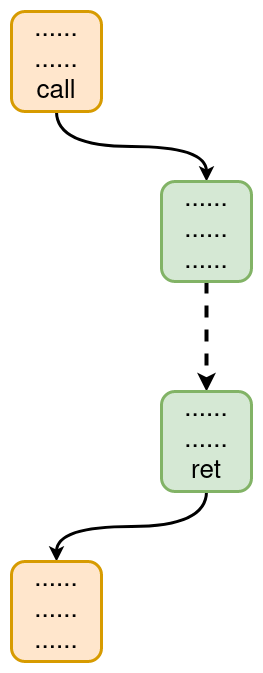
\includegraphics[width=.4\linewidth]{img/CallRetBefore.png}
		\caption{Original CFG}
	\end{subfigure}%
	\begin{subfigure}{.5\textwidth}
		\centering 	
		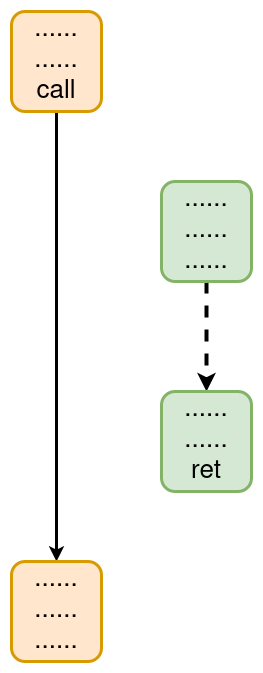
\includegraphics[width=.4\linewidth]{img/CallRetAfter.png}
		\caption{Transformed CFG}
	\end{subfigure}
	
	\caption{Transformation of the CFG around call/ret}
	\label{fig:callRet}
\end{figure}
 
\subsection{Finding the fetch}

\subsubsection{Basic Method}

The basic idea to find the fetch is to assume that all opcodes share the same basic block for the fetch, as in Figure \ref{fig:abstractVM:Centralized}.
Note that this is a somewhat restrictive assumption, albeit necessary for this method to work. Some VM implementations use a fetch block for each different opcode (see Figure \ref{fig:abstractVM:Decentralized}) : most notably CPython does so. This optimization ('computed-gotos') can thankfully be disabled when compiling CPython. In all my experiments I used this modified CPython version.
% todo : reference the CPython source file that implements computed gotos ?

\begin{figure}[htp]
	\centering
	\begin{subfigure}{.5\textwidth}
		\centering 	
		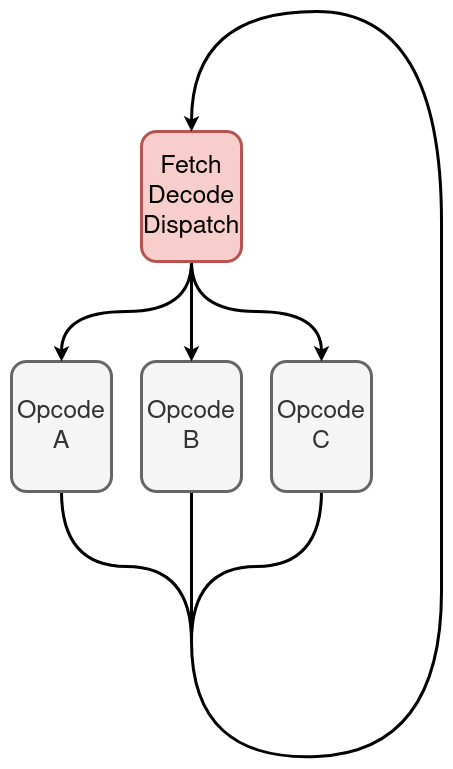
\includegraphics[width=.7\linewidth]{img/FetchCentralized.png}
		\caption{Centralized fetch}
		\label{fig:abstractVM:Centralized}
	\end{subfigure}%
	\begin{subfigure}{.5\textwidth}
		\centering 	
		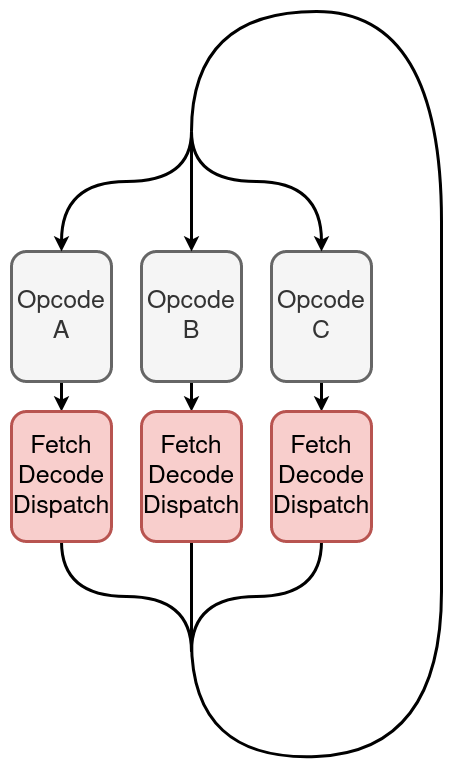
\includegraphics[width=.7\linewidth]{img/FetchDecentralized.png}
		\caption{Decentralized fetch ('computed-gotos')}
		\label{fig:abstractVM:Decentralized}
	\end{subfigure}
	\caption{Examples of VM control flow graphs}
	\label{fig:abstractVM}
\end{figure}

We thus build the CFG $\mathcal{C}$ and look for a basic block that :
\begin{itemize}
	\item is executed a large number of times (because it is shared between all opcodes).
	\item contains at least one instruction that reads a few bytes from memory (the fetch).
	\item has a large number of outgoing edges (the dispatch).
\end{itemize} 

Unfortunately, this method is too restrictive: the fetch, decode and dispatch aren't always in the same basic block in $\mathcal{C}$. There can be branches (e.g. to check for a termination condition, etc.) between the fetch and the dispatch, as shown in (ref to unfiltered cfg image). 

\subsubsection{Using the filtered CFG}

To handle this issue, we first filter out irrelevant detail from $\mathcal{C}$, and then hope that the fetch-decode-dispatch are in the same basic block in the new CFG $\mathcal{C}_{filtered}$. 

Given two parameters $exec\_blocks$ and $exec\_edges$, we build $\mathcal{C}_{filtered}$ as follows : 
\begin{itemize}
	\item For each block $B \in \mathcal{C}$, if $B$ is executed at least $exec\_blocks$ times, add $B$ to $\mathcal{C}_{filtered}$.
	\item For each edges $(E: B \rightarrow B') \in \mathcal{C}$, if $E$ is executed at least $exec\_edges$ times and both $B$ and $B'$ are executed at least $exec\_blocks$ times, add $E$ to $\mathcal{C}_{filtered}$.
\end{itemize}
We then apply a simple transformation on $\mathcal{C}_{filtered}$ to merge all blocks $B$ and $B'$ such that $next(B) = \{B'\}$ and $prev(B') = \{B\}$. During my experiments I had to tune the values of $exec\_blocks$ and $exec\_edges$, and found values around $1000$ to give satisfactory results. This method thus only works on Python programs that contain at least a few thousand opcodes.

The CFG $\mathcal{C}_{filtered}$ only retains the main structure of the graph, abstracting away the code paths rarely taken. However we might remove some or most of the opcode execution code from the graph : see figures \ref{fig:concreteVMFiltered} and \ref{fig:concreteVMOriginal} for a comparison between $\mathcal{C}$ and $\mathcal{C}_{filtered}$. The original CFG $\mathcal{C}$ is a good place to look for the dispatch, and $\mathcal{C}_{filtered}$ is the place to look for the fetch-decode-dispatch basic block. 

We thus look for a basic block in $\mathcal{C}_{filtered}$ that :
\begin{itemize}
	\item is executed a large number of times.
	\item contains at least one instruction that reads a few bytes from memory (the fetch).
	\item contains at least one instruction that has a large number of outgoing edges in $\mathcal{C}$.
\end{itemize}

Once we have found the fetch, it is easy to find the bytecode : we simply get the value read by the fetch. We can also divide the trace into chunks corresponding to each bytecode, and remove the irrelevant parts of the VM trace (initialization and finalization code) : we obtain a list of small traces for each bytecode.

\begin{figure}[htp]
	\centering 
	\begin{BVerbatim}
f = open("file", "w")
for i in range(1000):
	f.write(str(i))
	\end{BVerbatim}
	\caption{An example python program, used to generate the graphs in Figures 	\ref{fig:concreteVMFiltered} and \ref{fig:concreteVMOriginal}.}
	\label{fig:examplePythonProg}
\end{figure}

\begin{figure}[htp]
	\centering 	
	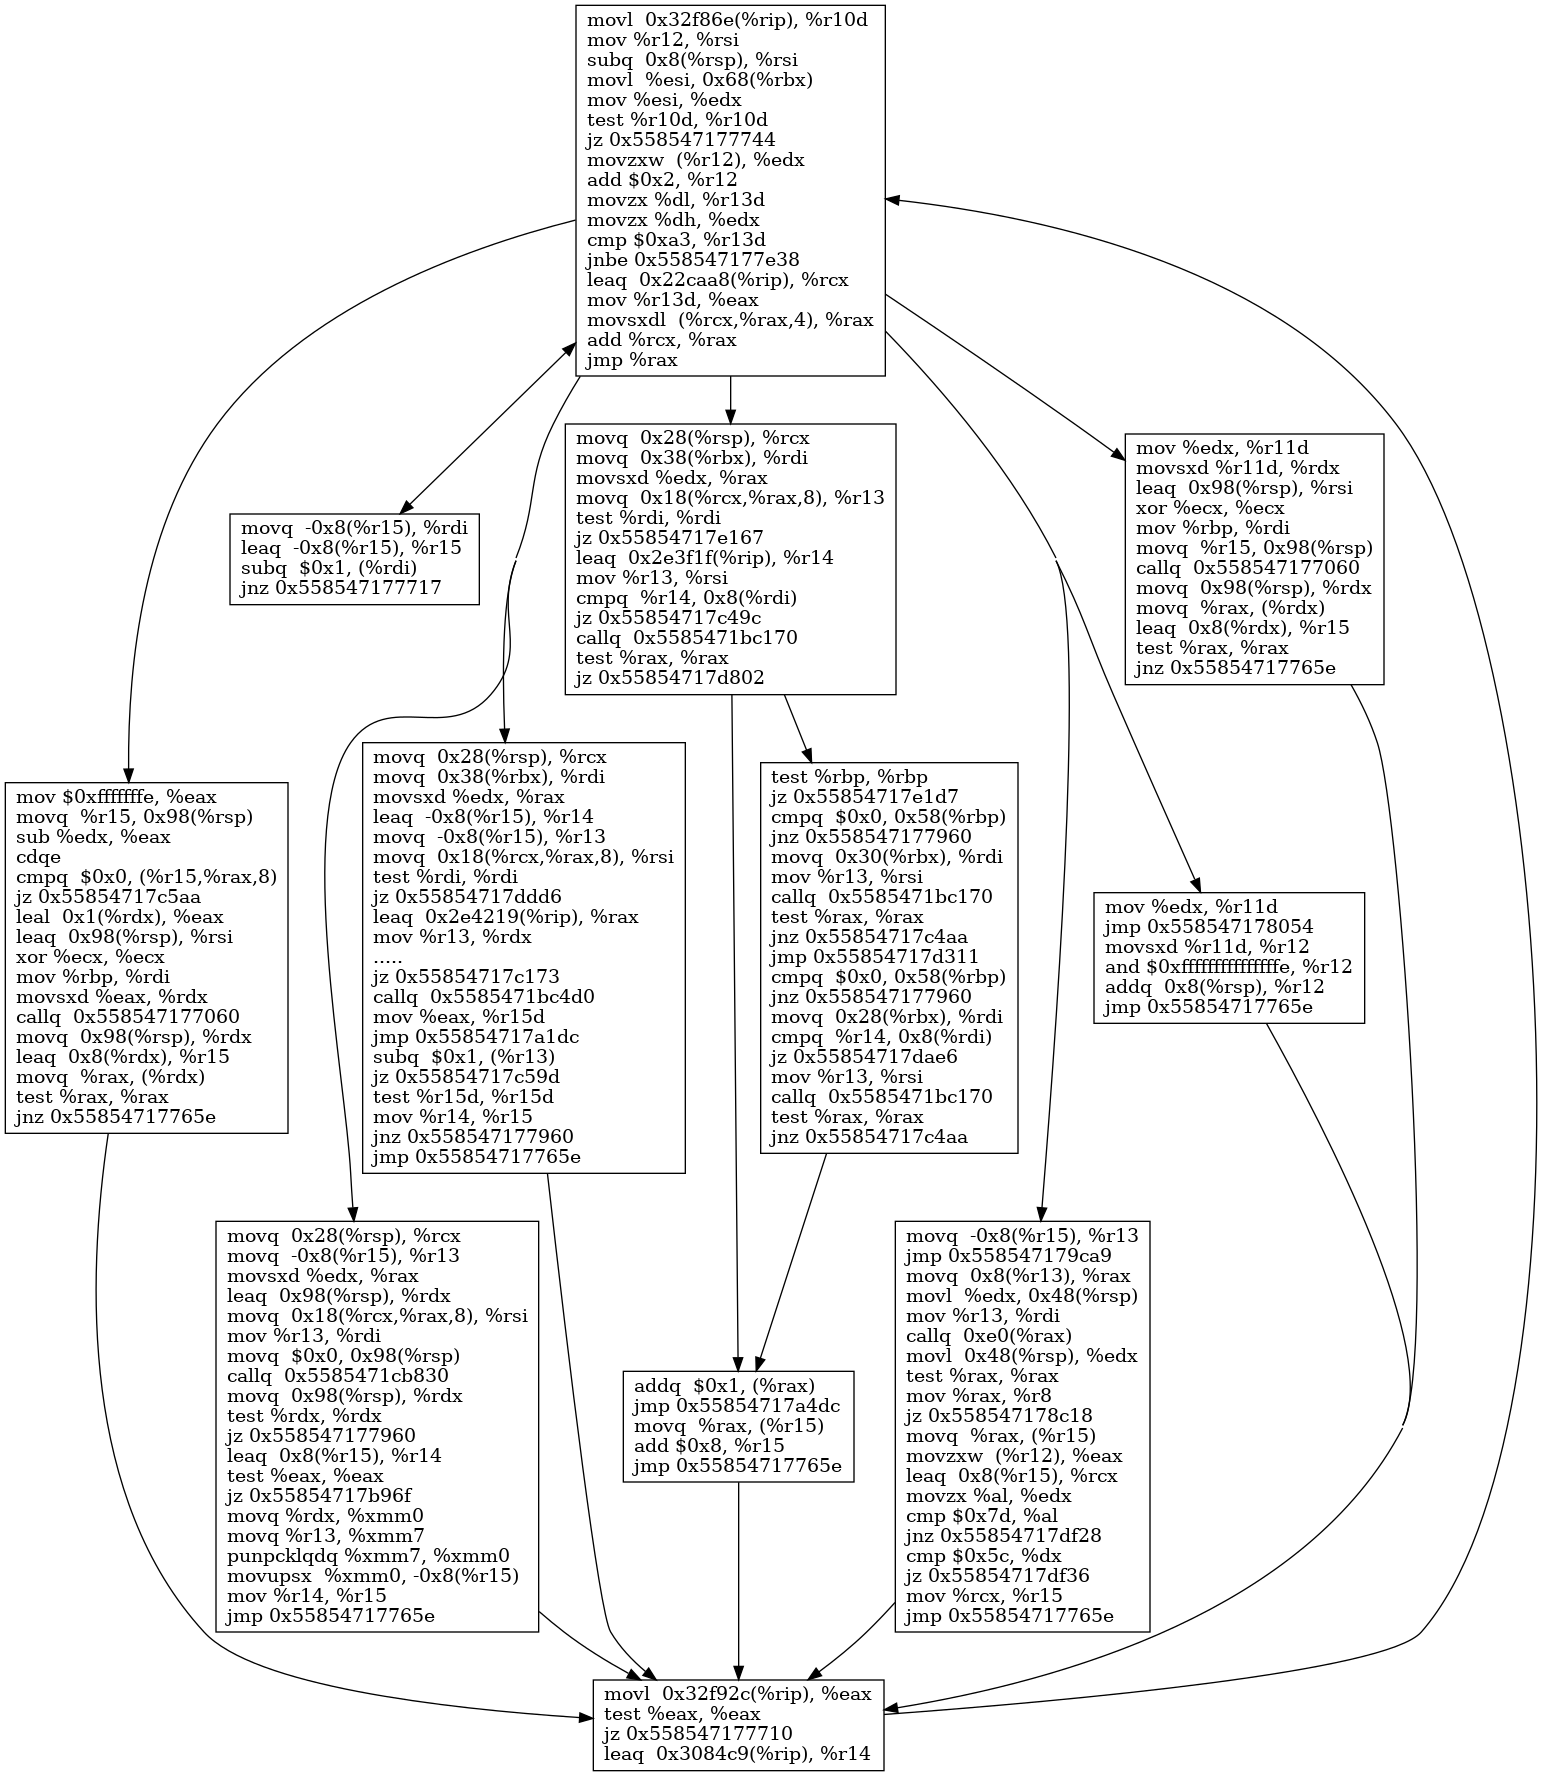
\includegraphics[width=\linewidth]{img/ConcreteVMFiltered.png}
	\caption{The function implementing the VM loop in $\mathcal{C}_{filtered}$, constructed from a trace of CPython running the program in Figure \ref{fig:examplePythonProg}. Notice how the fetch (movzxw (\%r12), \%edx)) and the dispatch (jmp \%rax) are in the same block (the top-most block), and that this block has relatively few outgoing edges.}
	\label{fig:concreteVMFiltered}
\end{figure}

\begin{figure}[htp]
	\centering 	
	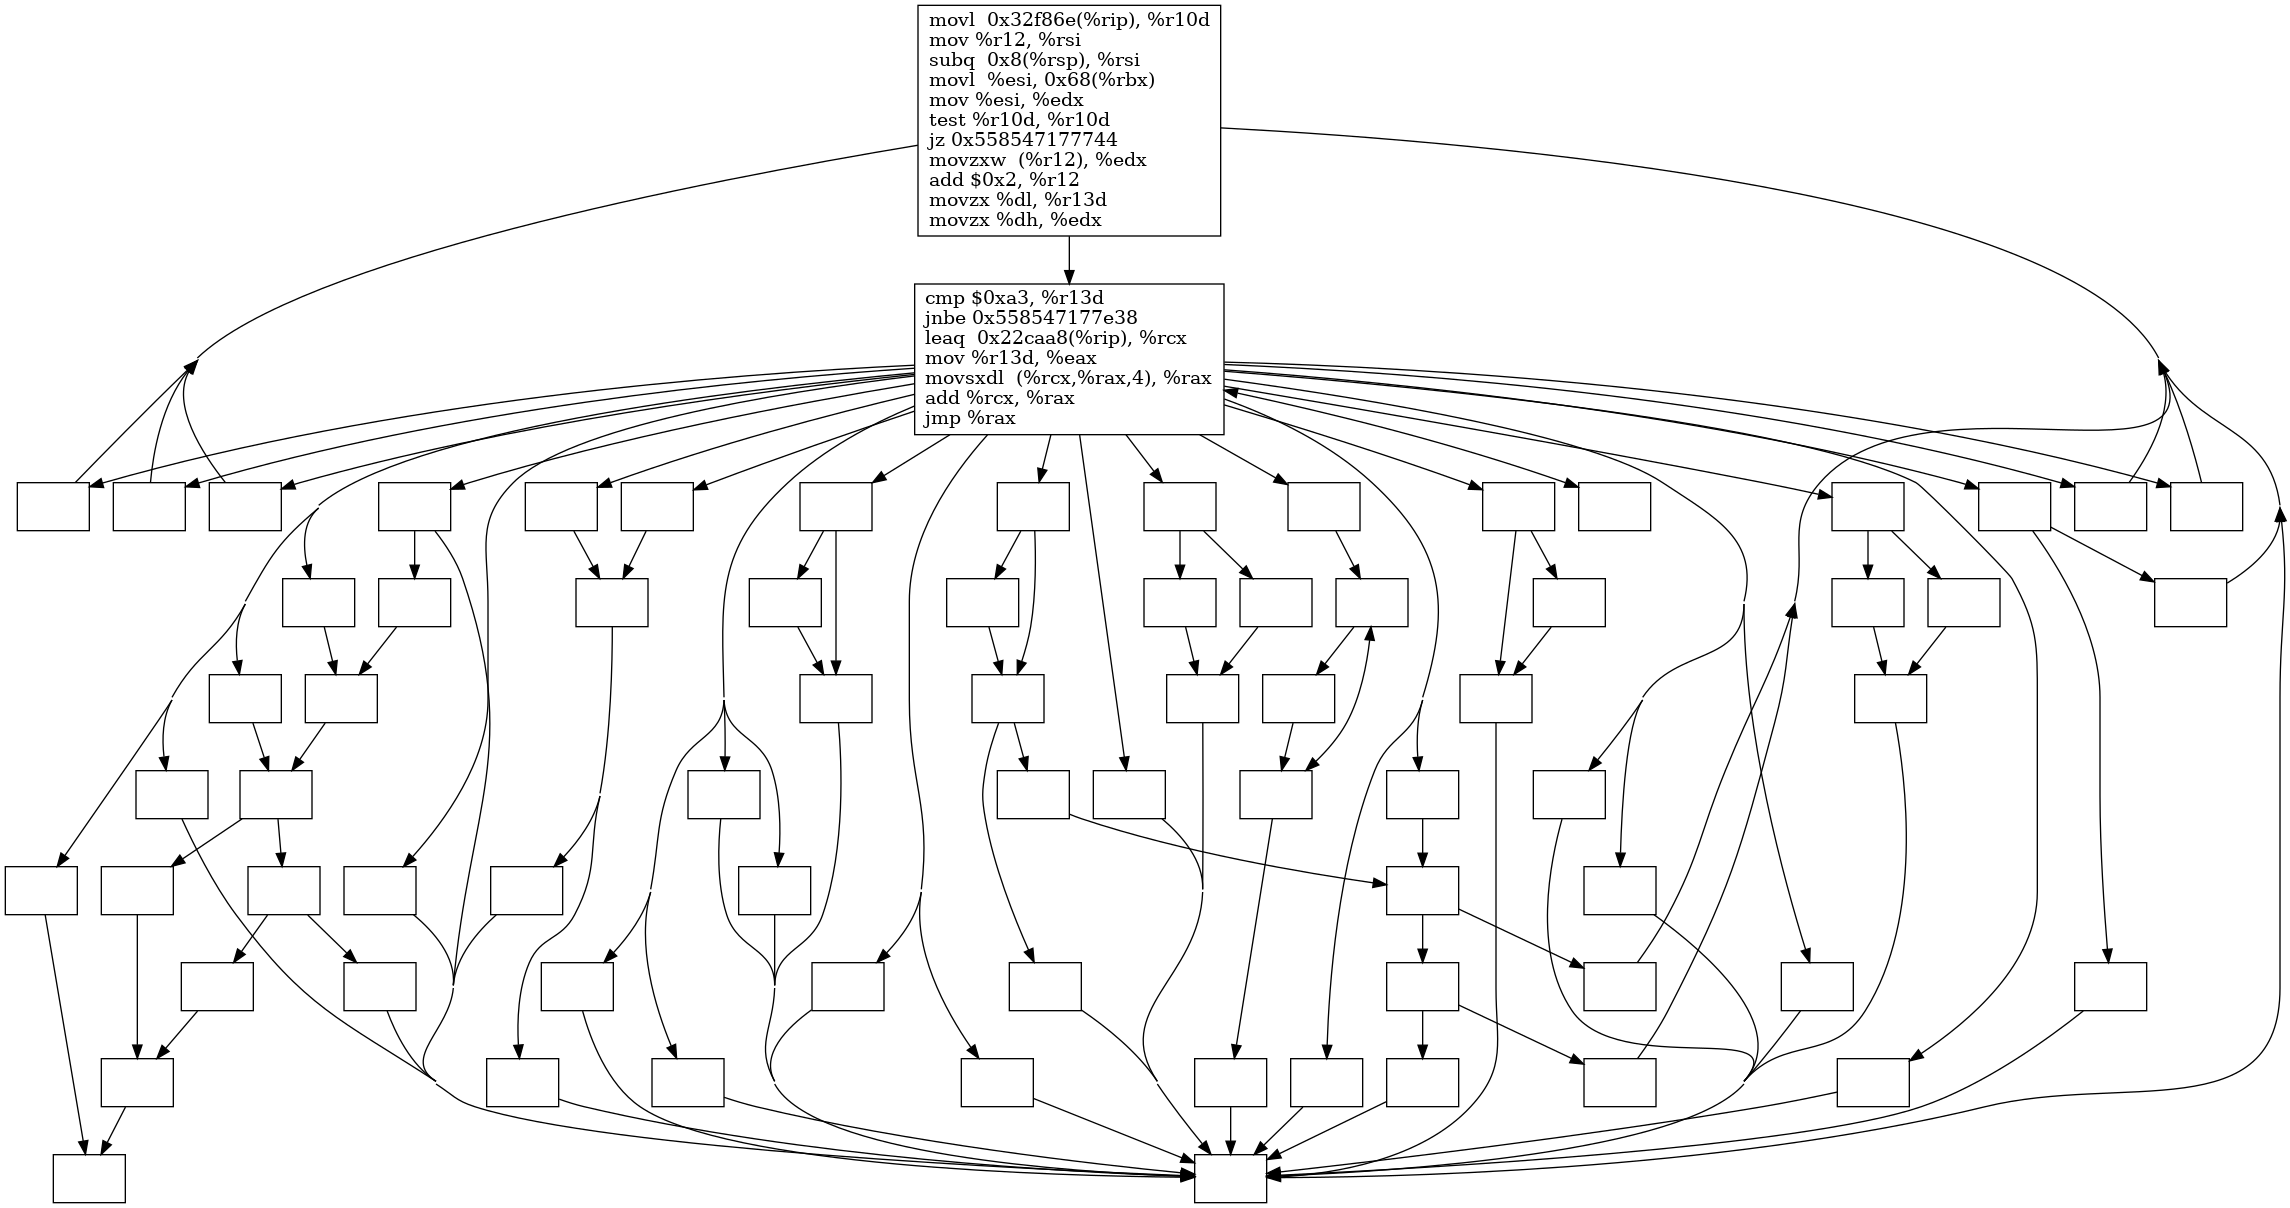
\includegraphics[width=\linewidth]{img/ConcreteVMOriginal.png}
	\caption{The function implementing the VM loop in $\mathcal{C}$, constructed from the same trace as in Figure \ref{fig:concreteVMFiltered}. Only the blocks implementing the fetch and the dispatch have their code shown. Notice how the fetch and the dispatch are in different blocks, and that the dispatch has many outgoing edges.}
	\label{fig:concreteVMOriginal}
\end{figure}

\section{Abstract VM model}

Before we can continue the analysis any further, we give ourselves an abstract VM model. While the previous section didn't assume much about the VM, this model follows more closely the Python VM.
\subsection{Definition}

We assume a stack-based VM, with no registers. It's internal state consists in :
\begin{itemize}
	\item a set of code blocks 
	\item a set of value stacks 
	\item a stack of frames.  
	\item pointers to the current frame ($fp$), the current bytecode ($ip$) and the top of the current value stack ($sp$)
\end{itemize}

A code block is a list of instructions. Each instruction is 2 bytes wide, the first byte being the opcode (example : ADD, POP, JMP) and the second byte being an argument. A code block contains all the code a given Python function can execute.

A value stack is a stack of Python values (objects). The contents of the stack are opaque to us. However all the values in the stack are contiguous in memory and of the same size.

Each frame corresponds to the execution of some Python function. A frame has its own code block and value stack.

The term "pointer" is intentionally vague : a pointer could be stored in a physical register or in a memory cell, it could contain the address of the object it points to or be an index into a list. During experiments I had to make additional assumptions about pointers, as will be explained in the following sections.

We will write $ptr \leftarrow f(ptr)$ where $f$ is any function and $ptr$ is $ip$, $sp$ or $fp$ to indicate that a given opcode changes the value of $ptr$ to $f(ptr)$.

\subsection{Finding the VM state}

We assume the state of the VM is valid at the fetch/dispatch block. At other points in the execution trace, the registers and memory cells used to store the VM state may be used for different purposes. Our goal is then to find the most information we can about the state before each bytecode.

\subsubsection{Finding $ip$}

Our method for finding the fetch gives us the instruction(s) that read the bytecode, and thus the address of the bytecode in memory : this gives us the value of $ip$ before each opcode, and also gives us access to the actual bytecode being executed (the value that is read by the fetch).

\subsubsection{Finding $fp$}

To find the frame pointers, we must make another assumption : that the C stack of the interpreter corresponds to the stack of the Python program it is running (remember we only look at the program state between bytecodes). Changes in $\%rsp$ should then give us the points at which the frame changes. Looking at registers that also change exactly and only at the same time as $\%rsp$ (and are also aligned on 8 bits) gives us additional frame pointers : pointers to some frame data (for instance, a C struct on the heap).

% todo : expand on this
Knowing the values of the frame pointers, we then tried to recognize the stack structure of frames, but some opcodes seem to operate on the stack of frame in non-standard ways : i.e. other than push or pop one, a even several, frame(s).

\subsubsection{Finding $sp$}

A first challenge is where to look for $sp$ : registers or memory ? It turns out it can be in both, depending on the interpreter (in a register for CPython, in memory for PyPy). Looking for $sp$ in registers is straightforward, as there are a very limited number of them. However memory is more complex : we can't scan through each memory cell. What we can hope for is that $sp$ is stored in a C struct pointed to by a frame pointer : $sp$ must be used very often, so requiring more than one pointer indirection to access it seems very inefficient. We thus look for $sp$ near addresses pointed to by frame pointers.  More precisely, we assume $sp$ will always be stored at $[fp + ofs]$ for $fp$ a frame pointer (whose value can change during the program execution) and $ofs$ a small constant offset (a multiple of 8).

To detect whether a location (register or memory cell) stores the value of $sp$, we take the list of values this location holds for each opcode. The basic idea is that many opcodes modify $sp$ in the same way : pop or push a few values. But we must be careful : we do not know whether $sp$ is stored as the address of the top stack cell, or as the index of the top stack cell, or something else. Depending on the case, a PUSH might increment $sp$ by $8$, $1$ or something else. The solution is to compute the alignment of $sp$, i.e. the largest power of $2$ that divides all the values in the list. We implement this idea as :
\begin{itemize}
	\item Compute the maximum consecutive number of times that $sp \leftarrow sp + k*align$ where $k$ is a small constant (e.g. $-2 \leq k \leq 2$). This number shouldn't change much with the size of the program (we check consecutive occurences) : we require it to be larger than a constant (e.g. $10$).
	\item Compute the maximum (not necessarily consecutive) number of times that $sp \leftarrow sp - align$, i.e. the number of POPs. This number should be proportional to the size of the program : we check it is larger than a percentage of the total opcode count (e.g. $10\%$).
\end{itemize}
The second test used is to distinguish between $sp$ and $ip$/$fp$: $ip$ and $fp$ might be stored in a similar way as $sp$, and pass the first test. 

\subsubsection{Code blocks}

We compute the code blocks by partitioning the bytecode instructions according to (the transitive closure of) the following relation. Two bytecode instructions are in the same code block if :
\begin{itemize}
	\item They are executed in the same frame (i.e. there is no frame change between two of their executions). This is because all instructions executed inside a frame are in the same Python function.
	\item They are close in memory. This is because different code blocks are likely to be far apart in memory. % todo : why ?
\end{itemize}


\section{Opcode semantics}

\subsection{Examples \& Challenges}

Once we have the values of $ip$ and $sp$ for each opcode, we try to attribute semantics to each opcode, i.e. characterize how they change the values of $ip$ and $sp$. One limitation of our 'shallow' description is that we do not known what values are stored on the stack : typical Python interpreters use the stack to store pointers to objects which we do not know the memory layout of. We thus can't differentiate between an ADD and a MUL operation for instance. All we can detect is the number of push/pops each opcode performs and how it changes the value of $ip$.

We would like to build semantics of the following form, e.g. for the simple case of an ADD opcode :
\begin{itemize}
	\item $ip \leftarrow ip + 2$
	\item $sp \leftarrow sp - 8$
\end{itemize}
Meaning that when we execute an ADD, $ip$ always increases by $2$ and $sp$ always decreases by $8$ (ADD pops its two arguments, pushes the result and advances to the next instruction). Remember that Python instructions are $2$ bytes long, so $ip + 2$ is the instruction directly following $ip$. However $sp$ can be the address of the top of the stack (in which case $sp - 8$ is the value directly under $sp$, since stack values are $8$ byte pointers) or can be something else, e.g. an index. In this case $sp$ will be aligned on $1$ rather than on $8$, and ADD would have the following semantics :
\begin{itemize}
	\item $ip \leftarrow ip + 2$
	\item $sp \leftarrow sp - 1$
\end{itemize}
Likewise, one could imagine a Python interpreter that grows the stack towards the bottom (CPython and PyPy both grow the stack towards the top), in which case it could become $sp \leftarrow sp + 1$. The precise semantics of an opcode thus depend on the particular interpreter we choose.

Another characteristic of our approach is that a single execution trace often doesn't give us enough information to find the most general semantics for an opcode. Take for example a conditional jump instruction such as POP\_JUMP\_IF\_TRUE, which performs a jump if the top of the stack is $true$ and otherwise advances to the next instruction. In a trace where each time we see this opcode the top of the stack is $false$, we can't detect that this is a conditional jump (or even a jump) and must give it the semantic $ip <- ip + 2$. We thus compute the most precise semantics for a given execution trace. 

Note that for a given opcode, several semantics may be acceptable. For instance the ADD opcode always has an argument equal to $0$ : thus we could characterize it by $ip \leftarrow ip + 2$ as well as by $ip \leftarrow ip + arg + 2$. In the second case we would interpret it as a relative jump, which it obviously isn't. I thus made the choice to only give the most 'general' characterization (in a sense I will define later on) for each opcode : ADD would thus be classified as $ip \leftarrow ip + 2$.

\subsection{Definition}

Building the $ip$-related semantics of an opcode is relatively straightforward. Most opcodes never change the current frame. For these, we five one of the following characterizations :
\begin{enumerate}
	\item Fall-through: $ip \leftarrow ip + k$. This corresponds to opcodes that don't alter the flow of control of the program.
	\item Relative jump : $ip \leftarrow ip + arg + k$.
	\item Absolute jump : $ip \leftarrow \textrm{block-start} + arg + k$.
	\item Conditional jump : $\textrm{either } ip \leftarrow ip + k_1 \textrm{ or } ip \leftarrow \textrm{block-start} + arg + k_2$. Note that we cannot find what the condition is, since this would require inspecting values in the stack.
\end{enumerate}
Here $k$, $k_1$ and $k_2$ are small constants (typically $-2 \leq k \leq 2$), $arg$ is the value of the argument of the opcode, and 'block-start' is the address of the first instruction in the current code block. 
The different characterizations are listed (top to bottom) from the most 'general' to the most precise : for each opcode, we give it the most 'general' characterization that is acceptable.

We didn't manage to find much about instructions that jump between frames, for lack of proper frame identification (we only know when frames change, not what frame we are in). We thus didn't characterize CALL or RET instructions. One additional difficulty is that CALL-like Python instructions don't always correspond to a change of frame. They are sometimes handled internally by the interpreter (e.g. calls to internal libraries such as I/O functions) : the next opcode in the trace is thus the fall-through instruction, and no frame change has been made.

Building the $sp$-related semantics is similar. Again, dealing with opcodes that change the current frame is too difficult, but for those that never change it, we give one of the following characterizations (from the most general to the least) :
\begin{enumerate}
	\item $sp \leftarrow sp + k$. This corresponds to most simple pop/push opcodes, as well as most binary operations (ADD, SUB, MUL, \dots).
	\item $sp \leftarrow sp \pm A*arg + k$. This corresponds to opcodes that either consume a number of values given by $arg$ (e.g. BUILD\_TUPLE) or produce a number of values given by $arg$ (e.g. UNPACK\_SEQUENCE).
\end{enumerate}
Here $k$ is a small constant (typically $-2 \leq k \leq 2$), $arg$ is the value of the argument of the opcode, and $A$ is the alignment of $sp$ (typically $1$ or $8$).


\begin{figure}[htp]
	\centering
	\begin{tabular}{|c|c|c|}
		\hline
		POP\_TOP & $ip \leftarrow ip + 2$ & $sp \leftarrow sp - 8$\\
		\hline
		MAKE\_FUNCTION & $ip \leftarrow ip + 2$ & $sp \leftarrow sp - 8$\\
		\hline
		BUILD\_SLICE & $ip \leftarrow ip + 2$ & $sp \leftarrow sp - 8$\\
		\hline
		DUP\_TOP & $ip \leftarrow ip + 2$ & $sp \leftarrow sp + 8$\\
		\hline
		ROT\_TWO & $ip \leftarrow ip + 2$ & $sp \leftarrow sp + 0$\\
		\hline
		UNARY\_NEGATIVE & $ip \leftarrow ip + 2$ & $sp \leftarrow sp + 0$\\
		\hline
		CALL\_FUNCTION\_KW & $ip \leftarrow ip + 2$ & $sp \leftarrow sp - 8*arg - 8$\\
		\hline
		EXTENDED\_ARG & $ip \leftarrow ip + 4$ & \\
		\hline
		BINARY\_MULTIPLY & $ip \leftarrow ip + 2$ & $sp \leftarrow sp - 8$\\
		\hline
		BINARY\_MODULO & $ip \leftarrow ip + 2$ & $sp \leftarrow sp - 8$\\
		\hline
		BINARY\_ADD & $ip \leftarrow ip + 2$ & $sp \leftarrow sp - 8$\\
		\hline
		BINARY\_SUBTRACT & $ip \leftarrow ip + 2$ & $sp \leftarrow sp - 8$\\
		\hline
		BINARY\_SUBSCR & $ip \leftarrow ip + 2$ & $sp \leftarrow sp - 8$\\
		\hline
		FORMAT\_VALUE & $ip \leftarrow ip + 2$ & $sp \leftarrow sp + 0$\\
		\hline
		BUILD\_STRING & $ip \leftarrow ip + 2$ & $sp \leftarrow sp - 8$\\
		\hline
		LOAD\_METHOD & $ip \leftarrow ip + 2$ & $sp \leftarrow sp + 8$\\
		\hline
		INPLACE\_ADD & $ip \leftarrow ip + 2$ & $sp \leftarrow sp - 8$\\
		\hline
		BINARY\_AND & $ip \leftarrow ip + 2$ & $sp \leftarrow sp - 8$\\
		\hline
		GET\_ITER & $ip \leftarrow ip + 4$ & $sp \leftarrow sp + 8$\\
		\hline
		LOAD\_BUILD\_CLASS & $ip \leftarrow ip + 2$ & $sp \leftarrow sp + 8$\\
		\hline
		POP\_BLOCK & $ip \leftarrow ip + 2$ & $sp \leftarrow sp + 0$\\
		\hline
		STORE\_NAME & $ip \leftarrow ip + 2$ & $sp \leftarrow sp - 8$\\
		\hline
		STORE\_ATTR & $ip \leftarrow ip + 2$ & $sp \leftarrow sp - 16$\\
		\hline
		LOAD\_CONST & $ip \leftarrow ip + 2$ & $sp \leftarrow sp + 8$\\
		\hline
		LOAD\_NAME & $ip \leftarrow ip + 2$ & $sp \leftarrow sp + 8$\\
		\hline
		BUILD\_TUPLE & $ip \leftarrow ip + 2$ & $sp \leftarrow sp - 8$\\
		\hline
		LOAD\_ATTR & $ip \leftarrow ip + 2$ & $sp \leftarrow sp + 0$\\
		\hline
		JUMP\_FORWARD & $ip \leftarrow ip + arg + 2$ & $sp \leftarrow sp + 0$\\
		\hline
		JUMP\_ABSOLUTE & $ip \leftarrow \textrm{ block-start } + arg + 0$ & $sp \leftarrow sp + 0$\\
		\hline
		POP\_JUMP\_IF\_FALSE & $ip \leftarrow \textrm{ block-start } + arg + 0$ & $sp \leftarrow sp - 8$\\
		\hline
		POP\_JUMP\_IF\_TRUE & 
		$ip \leftarrow 
		\left\{ 
		\begin{array}{ll}
		ip + 2 \\ 
		\textrm{block-start } + arg + 0
		\end{array}
		\right.$ & $sp \leftarrow sp - 8$\\
		\hline
		LOAD\_GLOBAL & $ip \leftarrow ip + 2$ & $sp \leftarrow sp + 8$\\
		\hline
		SETUP\_FINALLY & $ip \leftarrow ip + 2$ & $sp \leftarrow sp + 0$\\
		\hline
		LOAD\_FAST & $ip \leftarrow ip + 2$ & $sp \leftarrow sp + 8$\\
		\hline
		STORE\_FAST & $ip \leftarrow ip + 2$ & $sp \leftarrow sp - 8$\\
		\hline
	\end{tabular}
	\caption{Examples of opcode characterizations obtained with CPython.}
	\label{fig:}
\end{figure}



\begin{thebibliography}{9}
	\bibitem{tritondeobfs} 
	Jonathan Salwan, Sébastien Bardin and Marie-Laure Potet (2017).
	\\\textit{Désobfuscation binaire: Reconstruction de fonctions virtualisées}
	
	\bibitem{cpython}
	CPython : the official Python interpreter.
	\href{https://docs.python.org/3/}{\\\texttt{https://docs.python.org/3/}}
	
	\bibitem{pypy}
	PyPy : a Python interpreter written in Python.
	\href{https://doc.pypy.org/en/latest/}{\\\texttt{https://doc.pypy.org/en/latest/}}
	
	\bibitem{intelpin}
	Intel Pin : A Dynamic Binary Instrumentation Tool.
	\href{https://software.intel.com/content/www/us/en/develop/articles/pin-a-dynamic-binary-instrumentation-tool.html}{\\\texttt{https://software.intel.com/content/www/us/en/develop/articles/\\pin-a-dynamic-binary-instrumentation-tool.html}}
\end{thebibliography}
\end{document}


